\section{\heiti 方法}
\subsection{\heiti 总体流程}
\begin{multicols}{1}
	\begin{figure}[H]
		\centering
		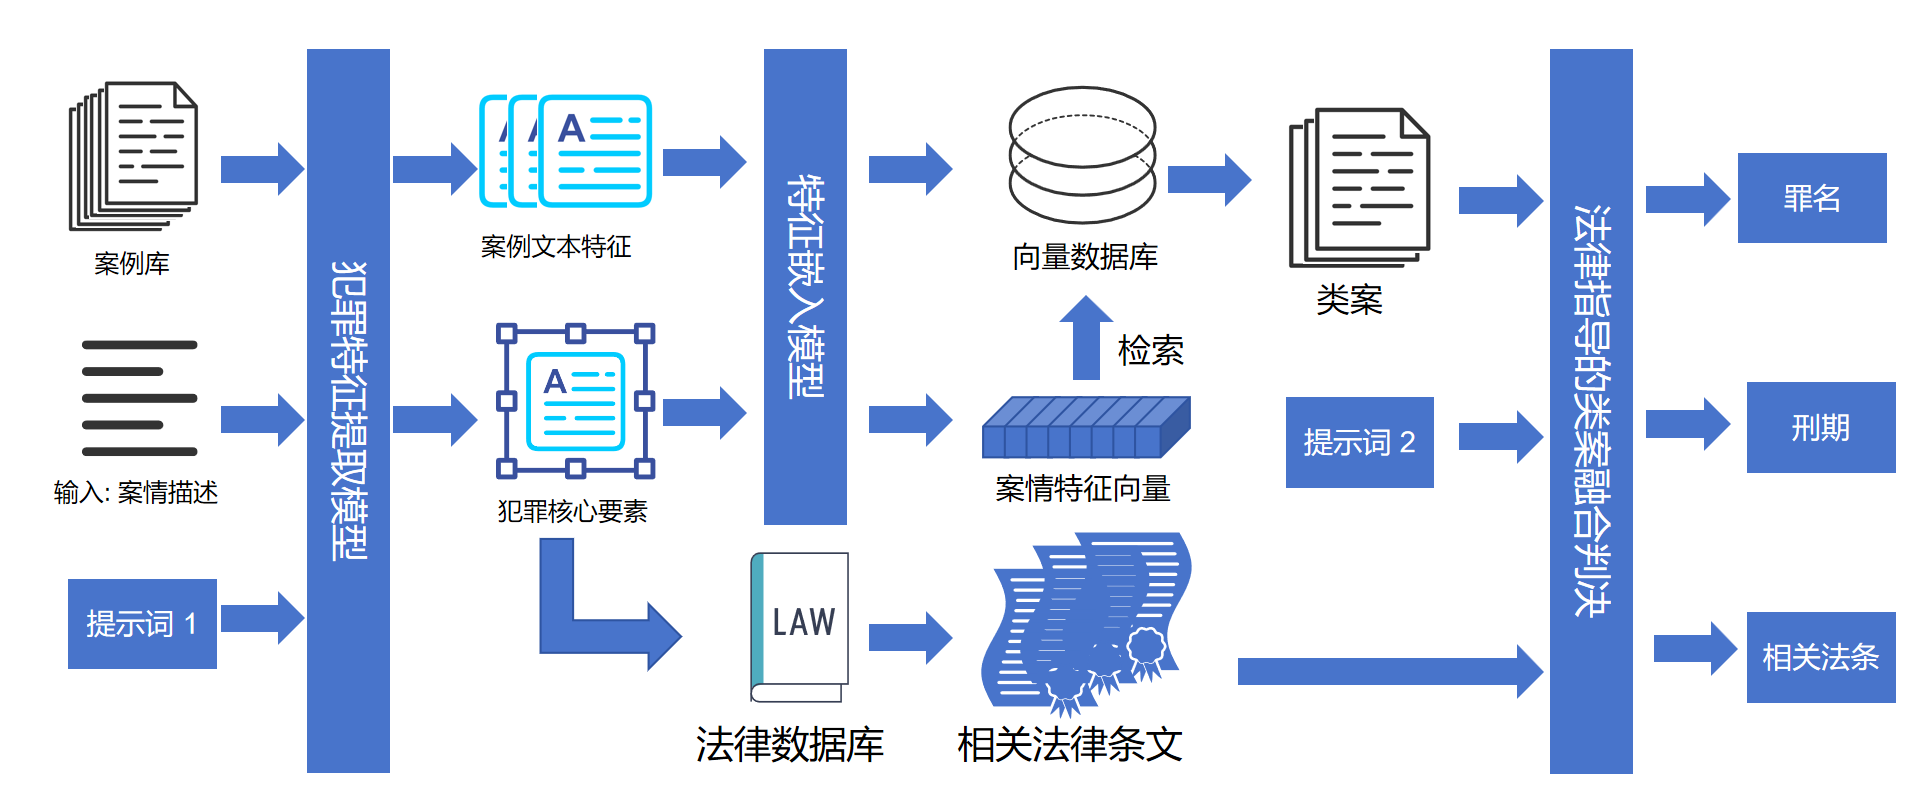
\includegraphics[width=1\textwidth]{fig/main.png}
		\caption{基于大语言模型, 法律引导的的案例融合方法, 用于司法判决预测流程}
		\label{fig:main}
	\end{figure}
\end{multicols}
本位提出的司法判决预测方法,其核心在于构建一个能够有效整合案件事实、法律法规及类案判例的智能推理框架。整体流程如图\ref{fig:main}所示。
首先,系统接收待判决案件的详细事实描述($C$),并利用预训练的大语言模型进行初步语义分析和关键信息抽取。该模型通过自然语言理解能力,从复杂的案情描述中识别并初步推断出罪名类别、犯罪构成要件(包括主体、主观、客体、客观)及证据特征等核心法律要素,形成结构化的犯罪特征表示($F$)。
其次,基于抽取的犯罪特征$F$,系统并行地从两个专门构建的法律知识库中检索相关信息。一方面,从权威的法律条文数据库中检索出与案件特征$F$高度相关的法律法规条款集合($L$)。另一方面,从海量的历史案例数据库中智能检索出与当前案件在罪名构成、事实情节和证据方面最为相似的判例集合($S$)。
最后,将原始案件事实描述$C$、检索到的相关法律条文$L$以及相似判例$S$共同作为上下文信息,输入至大语言模型,输出胡最终的判决结果。该模型作为核心推理引擎,通过整合这些多源异构信息,综合考量法律原则、司法解释及类案判例的指导作用,有效弥补了LLM在法律专业知识和复杂逻辑推理方面的固有局限性,显著增强了判决预测的专业性、准确性和可解释性。